\documentclass{article}

\usepackage[dutch]{babel}
\usepackage[margin=3cm]{geometry}
\usepackage{graphicx}
\usepackage{float}
\usepackage{caption}
\usepackage{hyperref}
\usepackage{amsmath}
\usepackage{wrapfig}
\usepackage[parfill]{parskip}

% fonts
\usepackage[T1]{fontenc}
\usepackage{helvet}
\renewcommand{\familydefault}{\sfdefault}

\graphicspath{{img/}}
 
\newcommand{\bold}[1]{\textbf{#1}}

%Define the listing package
\usepackage{listings} %code highlighter
\usepackage{upquote}
\usepackage{color} %use color
\definecolor{mygreen}{rgb}{0,0.6,0}
\definecolor{mygray}{rgb}{0.5,0.5,0.5}
\definecolor{mymauve}{rgb}{0.58,0,0.82}
\definecolor{lightgray}{rgb}{0.95, 0.95, 0.95}
\definecolor{darkgray}{rgb}{0.4, 0.4, 0.4}
\definecolor{purple}{rgb}{0.65, 0.12, 0.82}


\lstset{%
    % General design
    backgroundcolor=\color{lightgray},
    basicstyle={\small\ttfamily},   
    frame=l,
    % Code design
    identifierstyle=\color{black},
    keywordstyle=\color{blue}\bfseries,
    ndkeywordstyle=\color{greenCode}\bfseries,
    stringstyle=\color{red}\ttfamily,
    commentstyle=\color{darkgray}\ttfamily,
    % Code
    tabsize=4,
    showtabs=false,
    showspaces=false,
    showstringspaces=false,
    extendedchars=true,
    breaklines=true,
    % line-numbers
    xleftmargin={0.75cm},
    numbers=left,
    stepnumber=1,
    firstnumber=1,
    numberfirstline=true,
}

\lstdefinelanguage{CSS}{
    classoffset=0,
    keywords={accelerator,azimuth,background,background-attachment,
    background-color,background-image,background-position,
    background-position-x,background-position-y,background-repeat,
    behavior,border,border-bottom,border-bottom-color,
    border-bottom-style,border-bottom-width,border-collapse,
    border-color,border-left,border-left-color,border-left-style,
    border-left-width,border-right,border-right-color,
    border-right-style,border-right-width,border-spacing,
    border-style,border-top,border-top-color,border-top-style,
    border-top-width,border-width,bottom,caption-side,clear,
    clip,color,content,counter-increment,counter-reset,cue,
    cue-after,cue-before,cursor,direction,display,elevation,
    empty-cells,filter,float,font,font-family,font-size,
    font-size-adjust,font-stretch,font-style,font-variant,
    font-weight,height,ime-mode,include-source,
    layer-background-color,layer-background-image,layout-flow,
    layout-grid,layout-grid-char,layout-grid-char-spacing,
    layout-grid-line,layout-grid-mode,layout-grid-type,left,
    letter-spacing,line-break,line-height,list-style,
    list-style-image,list-style-position,list-style-type,margin,
    margin-bottom,margin-left,margin-right,margin-top,
    marker-offset,marks,max-height,max-width,min-height,
    min-width,-moz-binding,-moz-border-radius,
    -moz-border-radius-topleft,-moz-border-radius-topright,
    -moz-border-radius-bottomright,-moz-border-radius-bottomleft,
    -moz-border-top-colors,-moz-border-right-colors,
    -moz-border-bottom-colors,-moz-border-left-colors,-moz-opacity,
    -moz-outline,-moz-outline-color,-moz-outline-style,
    -moz-outline-width,-moz-user-focus,-moz-user-input,
    -moz-user-modify,-moz-user-select,orphans,outline,
    outline-color,outline-style,outline-width,overflow,
    overflow-X,overflow-Y,padding,padding-bottom,padding-left,
    padding-right,padding-top,page,page-break-after,
    page-break-before,page-break-inside,pause,pause-after,
    pause-before,pitch,pitch-range,play-during,position,quotes,
    -replace,richness,right,ruby-align,ruby-overhang,
    ruby-position,-set-link-source,size,speak,speak-header,
    speak-numeral,speak-punctuation,speech-rate,stress,
    scrollbar-arrow-color,scrollbar-base-color,
    scrollbar-dark-shadow-color,scrollbar-face-color,
    scrollbar-highlight-color,scrollbar-shadow-color,
    scrollbar-3d-light-color,scrollbar-track-color,table-layout,
    text-align,text-align-last,text-decoration,text-indent,
    text-justify,text-overflow,text-shadow,text-transform,
    text-autospace,text-kashida-space,text-underline-position,top,
    unicode-bidi,-use-link-source,vertical-align,visibility,
    voice-family,volume,white-space,widows,width,word-break,
    word-spacing,word-wrap,writing-mode,z-index,zoom},
    keywordstyle=\color{blue},
    classoffset=1,
    morekeywords={var, --*},
    keywordstyle=\color{mymauve},
    classoffset=0,
    sensitive=true,
    morecomment=[l]{//},
    morecomment=[s]{/*}{*/},
    morestring=[b]',
    morestring=[b]",
    moredelim=[is][\bfseries]{/@}{@/}, % Typesets characters between /@ and @/ delimeters in boldface.
}



\begin{document}

\begin{titlepage}
    \author{Tuur Vanhoutte}
    \title{Interaction design}
\end{titlepage}

\pagenumbering{gobble}
\maketitle
\newpage
\tableofcontents
\newpage

\pagenumbering{arabic}

\section{CSS Variables}

\subsection{Wat?}

\begin{itemize}
    \item CSS custom properties for cascading variables.
    \item CSS Variables = Custom Properties.
    \item Relatief nieuwe manier om veelgebruikte values om te zetten naar Variables.
    \item To keep consistency, set global variables for everything except layout values.
\end{itemize}

\subsection{Opbouw \& Syntax}

\subsubsection{Custom property: defining the variable}
Custom property: value

\begin{lstlisting}[language=CSS]
--my-cool-color: HotPink;
\end{lstlisting}

\subsubsection{Cascading variable: applying the variable}

Applying your custom property using the var() function

\begin{lstlisting}[language=CSS]
var(--my-cool-color)
\end{lstlisting}

\subsection{Syntax}

\begin{lstlisting}[language=CSS]
:root {
    --my-cool-color: HotPink;
}

p {
    color: var(--my-cool-color);
}

.foo {
    background-color: var(--my-cool-color);
}
\end{lstlisting}

\subsubsection{CSS Variables Are Case Sensitive}

\begin{lstlisting}[language=CSS]
:root {
    --foo: HotPink;
    --FOO: #BADA55;
}
p {
    color: var(--foo);
}
.foo {
    background-color: var(--FOO);
}
\end{lstlisting}


\subsubsection{This is wrong}

\begin{lstlisting}[language=CSS]
.test {
    --side: margin-top;
    var(--side): 20px
}
\end{lstlisting}

\subsubsection{Use the calc() function to do math}

\begin{lstlisting}[language=CSS]
:root {
    --whitespace: 20px;
    --whitespace-lg: var(--whitespace) * 2; /* won't work */
    --whitespace-lg: calc(var(--whitespace) * 2); /* correct */
}
\end{lstlisting}

\subsubsection{Kan ook shorthand values bevatten}

\begin{lstlisting}[language=CSS]
:root {
    --transition: all .1s ease-out;
}
a {
    transition: var(--transition);
}   
\end{lstlisting}

\subsubsection{Kan ook bestaan uit andere variables.}

\begin{lstlisting}[language=CSS]
:root {
    --transition-property: all;
    --transition-duration: .1s;
    --transition-timing-function: ease-out;
    --transition: var(--transtion-property) 
        var(--transition-duration) 
        var(--transition-timing-function);
}

a {
    transition: var(--transition);
}
\end{lstlisting}

\subsubsection{Default values}

\begin{lstlisting}[language=CSS]
.c-button {
    border: 1px solid var(--button-color, HotPink);
    background-color: transparent;
}
.c-button:hover {
    background-color: var(--button-color, HotPink);
}
.c-button--beta {
    --button-color: #BADA55;
}
\end{lstlisting}

\subsubsection{Default values with other variables}

\begin{lstlisting}[language=CSS]
:root {
    --color-pink: HotPink;
    --color-badass: #BADA55;
}
.c-button {
    border: 1px solid var(--button-color, var(--color-pink));
}
.c-button:hover {
    background-color: var(--button-color, var(--color-pink));
}
.c-button--beta {
    --button-color: var(--color-badass);
\end{lstlisting}

\subsection{Cascade}
CSS Variables Are Subject to the Cascade and Inheritance rules

\url{https://codepen.io/simoncoudeville-nmct/pen/BaBMGPZ}

\begin{lstlisting}[language=CSS]
:root {
    --my-cool-color: HotPink;
}
/* Alle elementen binnen de root waar je --
my-cool-color variable toepast zullen de
value HotPink overerven. */

p {
    color: var(--my-cool-color);
}

.foo {
/* Elke paragraaf in het element met
de class ".foo" krijgt de kleur #BADA55.*/

--my-cool-color: #BADA55;
}
\end{lstlisting}

\url{https://codepen.io/simoncoudeville-nmct/pen/aboMBop}

\subsubsection{CSS variables can be made conditional with @media and other conditional rules}

\begin{lstlisting}[language=CSS]
:root {
    --whitespace: 1em;
}
@media screen and (min-width: 768px) {
    :root {
        --whitespace: 2em;
    }
}
.c-card {
    padding: var(--whitespace);
}

\end{lstlisting}


\url{https://codepen.io/simoncoudeville-nmct/pen/JjXaQwB}

\subsubsection{Ideal for dark themes}

\begin{lstlisting}[language=CSS]
:root {
    --color: white;
    --background-color: black
}
@media (prefers-color-scheme: dark) {
    :root {
    --color: black;
    --background-color: white
    }
}
.html {
    background-color: var(--background-color);
    color: var(--color);
}
\end{lstlisting}

\url{https://codepen.io/simoncoudeville-nmct/pen/eYOxbPp}

\subsection{Hoisting}
= Accessing a Variable First and Declaring Later

\begin{lstlisting}[language=CSS]
body{
    background: var(--bg-fill);
}
:root{
    --bg-fill: green;
}

\end{lstlisting}

\subsection{Scoped variables}

Twee soorten:
\begin{itemize}
    \item Global Scoped Variables
    \item Local Scoped Variables
\end{itemize}

\subsubsection{Global scoped variables}

\begin{lstlisting}[language=CSS]
:root {
    --global-color: black;
}
\end{lstlisting}
\begin{itemize}
    \item :root is a CSS pseudo-class selector used to select the element that represents the root of the document.
    \item :root is hetzelfde als html maar is specifieker
    \item :root = html
    \item :root > html
\end{itemize}

\url{https://codepen.io/simoncoudeville-nmct/pen/OJLBKXq}

Global variables kan je overal hergebruiken en overschrijven. Ideaal dus voor values die veel hergebruikt worden:

\begin{itemize}
    \item colors
    \item whitespace
    \item border-radius
    \item transitions
    \item \dots
\end{itemize}

\subsubsection{Local scoped variables}
\begin{itemize}
    \item Local scoped variables worden gedeclareerd binnen een specifieke selector.
    \item Local scoped variables hebben access tot global scoped variables.
    \item Ideaal voor components.
\end{itemize}

\begin{lstlisting}[language=CSS]
.alert {
    --alert-color: #222;
    color: var(--alert-color);
    border-color: var(--alert-color);
}
:root {
    --global-fontSize: 16px;
}
.c-button {
    --button-fontSize: var(--global-fontSize);
    font-size: var(--button-fontSize);
}
\end{lstlisting}


\subsection{Naming system}

\subsubsection{The two-level theming system}

Systeem om global variables te gebruiken in local variables.

\subsubsection{Global level}

De hoofdreden om global variables te hebben is consistentie.

They are prefixed with the word global and follow this formula:

-{}-global-{}-concept-{}-modifier-{}-state-{}-propertyCamelCase

\begin{itemize}
    \item a concept is something like a spacer, main-title or text
    \item a state is something like hover, or expanded
    \item a modifier is something like sm, or lg
    \item and a propertyCamelCase is something like backgroundColor or fontSize
\end{itemize}

\subsubsection{Local level}

They follow this formula: 

-{}-block\_\_element-{}-modifier-{}-state-{}-propertyCamelCase

\begin{itemize}
    \item The block\_\_element-{}-modifier selector name is something like alert\_\_actions or alert--primary
    \item a state is something like hover or active
    \item The value of component scoped variables is always defined by a global variable.
\end{itemize}


\begin{lstlisting}[language=CSS]
.c-alert {
    /* Component scoped variables are always defined by global variables */
    --c-alert--Padding: var(--global--spacer--md);
    --c-alert--primary--BackgroundColor: var(--global--primary-color);
    --c-alert__title--FontSize: var(--global--secondary-title--fontSize);
    /* --block--propertyCamelCase */
    padding: var(--c-alert--padding);
}

/* --block--state--propertyCamelCase */
.c-alert--primary {
    background-color: var(--c-alert--primary--backgroundColor);
}

/* --block__element--propertyCamelCase */
.c-alert__title {
    font-size: var(--c-alert__title--fontSize);
}
\end{lstlisting}

\subsection{Herhalingsvragen}

\begin{itemize}
    \item Hoe worden CSS variables nog genoemd?
    \item Hoe worden CSS variables opgebouwd?
    \item Wat is CSS Hoisting?
    \item Wat is het verschil tussen global en local variables?
\end{itemize}

\url{https://codepen.io/simoncoudeville-nmct/pen/vYBbbXz?editors=1100}

\section{Forms}

\subsection{Form}
\begin{itemize}
    \item HTML forms are a very powerful tool for interacting with users
    \item Groot deel van een digitale interface
    \item In veel vormen en maten
\end{itemize}

\subsubsection{Voorbeelden}
\begin{itemize}
    \item Nieuwe repo maken op github
    \item Profiel aanmaken
    \item Route kiezen DeLijn
    \item \dots
\end{itemize}

\subsubsection{Basic form syntax}

\begin{lstlisting}[language=HTML]
<form action="">
    <input type="">
    ...
    Submit
</form>
\end{lstlisting}

\bold{Maak geen forms zonder (submit) button!} Zonder (submit) button kan je niet op enter duwen

\subsection{Input types}

\begin{itemize}
    \item Alle input types: \url{https://www.w3schools.com/tags/att_input_type.asp}
    \item Dit zijn de belangrijkste types die je moet kennen:
    \begin{itemize}
        \item Text-achtigen
        \item Time-achtigen
        \item Option-achtigen
        \item Textarea
        \item Select
        \item Range
        \item Hors catégorie
    \end{itemize} 
\end{itemize}

\subsubsection{HTML5 input types}

\begin{itemize}
    \item Browser validatie
    \item Smartphone keyboard verandert
    \item Testen op je smartphone: 
    
    \url{https://mobiforge.com/design-development/html5-mobile-
    web-forms-and-input-types}
    \item Live demo: \url{https://codepen.io/simoncoudeville-nmct/pen/gQYqBY}
\end{itemize}

\subsubsection{Text-achtigen}

\begin{itemize}
    \item Zien er visueel ongeveer hetzelfde uit
    \item Op smartphones: keyboard veranderd op basis van welk type de input is
    \item \bold{text} - basis input type voor HTML5 input types
    \item \bold{password} - vervangt de letters door bolletjes
    \item \bold{email} - valideert de browser enkel als je een correct e-mail adres invult
    \item \bold{number}
    \begin{itemize}
        \item Aanvaardt enkel nummers
        \item Heeft pijltjes om te vermeerderen of te verminderen
    \end{itemize}
    \item \bold{tel} - telefoonnummers
\end{itemize}

\subsubsection{Time-achtigen}

\begin{itemize}
    \item Zien er visueel ongeveer hetzelfde uit als de text-achtigen
    \item date - toont een native date picker
    \item week - toont een variant van de native date picker
    \item month - toont een variant van de native date picker
    \begin{itemize}
        \item Vooral date zal je kunnen gebruiken.
    \end{itemize}
    \item number - aanvaardt enkel nummers
    \item tel - handig voor mobile
\end{itemize}

\begin{figure}[H]
    \centering
    \includegraphics[width=0.5\textwidth]{input-date-time.png}
    \caption{<input type="date"> en <input type="time"> op smartphones}
\end{figure}

\subsubsection{Option-achtigen}

\bold{checkbox}

\begin{itemize}
    \item Meerdere keuzes mogelijk uit een aantal keuzes
    \item Of kan alleen bestaan
\end{itemize}

\bold{radio(button)}

\begin{itemize}
    \item Slechts 1 keuze mogelijk uit een aantal keuzes
    \item Kan niet alleen bestaan, altijd in en group
    \item Gekoppeld aan elkaar door het name attribuut
    \item Niet voor enkele binaire keuzes
    \item Kan je ook customizen met CSS
\end{itemize}

Geschiedenis van de radio-button: \url{https://www.jitbit.com/radio-button/}

\begin{figure}[H]
    \centering
    \includegraphics[width=0.4\textwidth]{radiobuttons.png}
    \includegraphics[width=0.3\textwidth]{checkboxes.png}
    \caption{}
\end{figure}

\bold{Laat een checkbox er nooit uitzien als een radio button en omgekeerd!}

\subsection{Checkbox or toggle?}
\begin{figure}[H]
    \centering
    \includegraphics[width=0.2\textwidth]{toggle-switch.png}
    \caption{Links: toggle switch, rechts: checkbox}
\end{figure}

\subsubsection{Checkbox}
\begin{itemize}
    \item Checked of niet
    \item Heeft nog confirmatie nodig
    \item Meerdere opties die bij elkaar horen
    \item Checken van sub options (intermediate state)
    \item Enkele ja/nee optie
\end{itemize}

\subsubsection{Toggle switch = veredelde checkbox}
\begin{itemize}
    \item Aan of af zetten
    \item Instant response zonder confirmatie
    \item Afzonderlijke features of settings
    \item Enkele aan/af beslissing
\end{itemize}

\subsubsection{Voorbeelden}

\begin{figure}[H]
    \centering
    \includegraphics[width=0.5\textwidth]{toggle-ex-1.png}
    \caption{De opties die een directe reactie vereisen kunnen het best geselecteerd worden met een toggle switch.}
\end{figure}

\begin{figure}[H]
    \centering
    \includegraphics[width=0.5\textwidth]{toggle-ex-2.png}
    \caption{Checkboxes hebben de voorkeur wanneer een expliciete actie vereist is om instellingen toe te passen.}
\end{figure}

\begin{figure}[H]
    \centering
    \includegraphics[width=0.5\textwidth]{toggle-ex-3.png}
    \caption{Selecteren van meerdere opties in een lijst biedt betere ervaring met checkboxes.}
\end{figure}

\begin{figure}[H]
    \centering
    \includegraphics[width=0.5\textwidth]{toggle-ex-4.png}
    \caption{Indeterminate state wordt het best voorgesteld met een checkbox. (zie `All' aan de linkerkant)}
\end{figure}

\begin{figure}[H]
    \centering
    \includegraphics[width=0.5\textwidth]{toggle-ex-5.png}
    \caption{Afzonderlijke features of settings zijn dan weer logischer met toggle switches.}
\end{figure}

\begin{figure}[H]
    \centering
    \includegraphics[width=0.5\textwidth]{toggle-ex-6.png}
    \caption{Een enkele ja/nee optie is logischer met een checkbox.}
\end{figure}

\begin{figure}[H]
    \centering
    \includegraphics[width=0.5\textwidth]{toggle-ex-7.png}
    \caption{Een enkele aan/af beslissing is logischer met een toggle switch.}
\end{figure}

\subsubsection{Toggle Switch of Toggle Button?}

\bold{Toggle buttons = soort van veredelde radio button of meerdere buttons}

\begin{itemize}
    \item Contextual state
    \item Heeft invloed op het huidige scherm
    \item Opposing options
\end{itemize}


\bold{Toggle switch = veredelde checkbox}
\begin{itemize}
    \item System state
    \item Heeft invloed op de volledige app
    \item Binary options
\end{itemize}

\begin{figure}[H]
    \centering
    \includegraphics[width=0.5\textwidth]{toggle-buttons.png}
    \caption{}
\end{figure}

\begin{figure}[H]
    \centering
    \includegraphics[width=0.5\textwidth]{toggle-buttons2.png}
    \caption{Switches are for binary options, not opposing options.}
\end{figure}

\subsection{Textarea}
\begin{itemize}
    \item <textarea>
    \item Geen input type, apart element
    \item Multi-line text input control
    \item De gebruiker kan optioneel de grootte aanpassen van het tekstvak
\end{itemize}

\subsection{Select}
\begin{itemize}
    \item <select>
    \item Geen input type, apart element
    \item dropdown list
    \item De <option> tags binnen het <select> element definieren de beschikbare options in de lijst
    \item \bold{Native select} behouden als je designt: geen eigen element proberen te maken $\Rightarrow$ gebruiksvriendelijker op smartphone.
\end{itemize}

\subsection{Range}
\begin{itemize}
    \item Slider control
    \item Voor nummers
    \item Default range van 0 tot 100
    \begin{itemize}
        \item restrictions zijn mogelijk met max, min en step attributes
    \end{itemize}
\end{itemize}

\subsection{Hors catégorie}
\begin{itemize}
    \item \bold{file} - file upload
    \item \bold{hidden} - voor developers
    \item \bold{color} - toont een color picker
\end{itemize}


\subsection{Attributes}
= Eigenschappen van de input

\begin{itemize}
    \item bv: type, value, id, name, \dots
    \item Alle attributes: \url{https://www.w3schools.com/html/html_form_attributes.asp}
\end{itemize}

\subsubsection{Minimum attributes}
\begin{itemize}
    \item \bold{type} - defineert het type input (duh!)
    \item \bold{name}
    \begin{itemize}
        \item Voor developers
        \item Zorgt er voor dat je weet wat je waar ingevuld hebt
        \item Ook om radio buttons aan elkaar te koppelen
        \item \bold{Dus altijd een name voorzien!}
    \end{itemize}
\end{itemize}

\subsubsection{Veelgebruikte attributes}

\begin{itemize}
    \item \bold{value}
    \begin{itemize}
        \item Kan je gebruiken om een default value in te geven
        \item Indien leeg wordt dit wat je hebt ingevuld
    \end{itemize}
    \item \bold{placeholder}
    \begin{itemize}
        \item hint
        \item voorbeeld van de wat de value moet zijn
        \item Verdwijnt automatisch als je begint te typen
        \item Placeholder nooit gebruiken als alternatief voor een label!
    \end{itemize}
\end{itemize}

\begin{figure}[H]
    \centering
    \includegraphics[width=0.5\textwidth]{veelgebruikte-attributes.png}
    \caption{}
\end{figure}

\subsubsection{Lege attributes}

\begin{itemize}
    \item Hebben geen value
    \item Zijn waar of onwaar
    \item CSS pseudo classes
    \item Veel gebruikt:
    \begin{itemize}
        \item \bold{Checked} - radio options \& checkboxes
        \item \bold{Required} - voor browservalidatie
        \item \bold{Disabled} - kan je niet aanpassen en wordt ook niet gesubmit
        \item \bold{Readonly} - kan je niet aanpassen maar wordt wel gesubmit
        \item \bold{Autofocus} - focust automatisch op het input type
    \end{itemize}
\end{itemize}

\begin{figure}[H]
    \centering
    \includegraphics[width=0.5\textwidth]{lege-attributes.png}
    \caption{required}
\end{figure}


\subsection{Labels}
\begin{itemize}
    \item Gekoppeld aan een input
    \item Usability improvement: toggles the input
    \item Elke input moet een label hebben!
    \item Niet vervangen door placeholder!
    \begin{itemize}
        \item In een lang ingevuld formulier weet je op den duur niet meer wat je waar moet invullen
        \item Alternatief: floating label pattern:
        \item \url{https://dribbble.com/shots/3429471-Floating-label-input-field}
        \item \url{https://codepen.io/soulrider911/pen/ugnyl}
    \end{itemize}
\end{itemize}

\subsubsection{Label koppelen aan input - Manier 1}

\begin{itemize}
    \item Met for en id
    \item Label text is apart aanspreekbaar met CSS.
\end{itemize}

\begin{lstlisting}[language=HTML]
<label for="input_id">label text</label>
<input type="text" name="whatever" id="input_id">
\end{lstlisting}



\subsubsection{Label koppelen aan input - Manier 2}
\begin{itemize}
    \item Geen for en id nodig (maar wel altijd aangeraden)
    \item Label text is niet aanspreekbaar met CSS.
\end{itemize}

\begin{lstlisting}[language=HTML]
    <label>
        label text
        <input type="text" name="whatever" id="input_id">
    </label>
    \end{lstlisting}


\subsection{Buttons}
\bold{Elk formulier moet een button hebben! (Binnen de form tag)}

\subsubsection{Als input type}

\begin{lstlisting}[language=HTML]
<input type="submit" value="verzenden">
<input type="button" value="verzenden">
\end{lstlisting}

\subsubsection{Als button element}

\begin{lstlisting}[language=HTML]
<button>verzenden</button>
\end{lstlisting}

\bold{Gebruik het button element!}

\begin{lstlisting}[language=HTML]
<button class="c-button">
    <span class="c-button__label">Verzenden</span>
    <svg class="c-button__symbol>...</svg>
</button>
\end{lstlisting}

\subsection{States}
\begin{enumerate}
    \item :hover
    \item :active
    \item :focus
\end{enumerate}

Deze volgorde in de CSS is zeer belangrijk!

\url{https://codepen.io/simoncoudeville-nmct/pen/oNxJbea}

\subsubsection{:hover}

CSS declarations worden geactiveerd\dots

\begin{itemize}
    \item Op pc: wanneer een gebruiker de muis over een element beweegt.
    \item Op mobiele toestellen: als een gebruiker een element "induwt" en "loslaat" en er geen specifieke focus of active styles zijn gedeclareerd of als :hover na :focus of :active komt.
\end{itemize}

\subsubsection{:active}

\begin{itemize}
    \item CSS declarations worden geactiveerd wanneer een gebruiker met de muis klikt.
    \item CSS declarations worden geactiveerd op mobiele toestellen als een gebruiker een element "induwt".
    \item Extra feedback feedback
\end{itemize}

\subsubsection{:focus}
\begin{itemize}
    \item Focus toont duidelijk welk element op de pagina keyboard events kan ontvangen
    \item Het element dat gefocust is heeft een duidelijke focus ring of outline of een andere visuele clue die de designer voorzien heeft.
    \item Welk element gefocust is kan je bedienen met het keyboard via tab of shift tab
    \item De volgorde is de tab order
    \item Interactieve HTML elementen zoals input, buttons, links zijn impliciet focusbaar. Ze worden automatisch aan de tab order toegevoegd.
    \item Paragrafen, divs, images enz\dots zijn niet focusbaar
\end{itemize}

\begin{figure}[H]
    \centering
    \includegraphics[width=0.4\textwidth]{focus.png}
    \includegraphics[width=0.2\textwidth]{focus2.png}
    \caption{}
\end{figure}

\begin{itemize}
    \item Voorbeeld van een form waar je niet op kan klikken, te bedienen met de tab-toets
    \item \url{http://udacity.github.io/ud891/lesson2-focus/01-basic-form/}
    \item Probeer eens een ticket te boeken voor\dots
    \begin{itemize}
        \item een round trip
        \item van Sydney naar Melbourne
        \item van 12 oktober tot 23 oktober 2018
        \item aan het venster
        \item en je wil geen promotionele aanbiedingen
    \end{itemize}
    \item Met tab, de pijltjes, spatie voor checkbox, \dots
\end{itemize}

\subsection{Validation}

\begin{itemize}
    \item Voorkom dat gebruikers fouten maken
    \item Als ze dan toch fouten maken en kunnen submitten:
    \begin{itemize}
        \item Verzorg duidelijke foutboodschappen
        \item Zet foutboodschappen inline bij hun input
    \end{itemize} 
\end{itemize}

\subsubsection{Client side validation}
\begin{itemize}
    \item Voor dat data wordt doorgestuurd naar de server
    \item Instant response
    \item HTML5 validation
    \item \begin{itemize}
        \item Required, valid \& invalid pseudo classes om instant te tonen of het juist is of niet.
        \item \url{https://codepen.io/chriscoyier/pen/JXgKjb}
    \end{itemize}
    \item + Javascript validation omdat je html kan aanpassen in developers tools
\end{itemize}

\subsubsection{Server side validation}
\begin{itemize}
    \item Voordat het opgeslaan wordt in de database
    \item Laatste
\end{itemize}

\subsubsection{Voorbeelden}
\begin{figure}[H]
    \centering
    \includegraphics[width=0.45\textwidth]{validation1.png}
    \includegraphics[width=0.45\textwidth]{validation2.png}
    \caption{}
\end{figure}

\begin{figure}[H]
    \centering
    \includegraphics[width=0.35\textwidth]{validation3.png}
    \caption{}
\end{figure}

\begin{figure}[H]
    \centering
    \includegraphics[width=0.45\textwidth]{validation4.png}
    \includegraphics[width=0.45\textwidth]{validation5.png}
    \caption{Waar validation gebruiken?}
\end{figure}


\subsection{Extra (geen vragen op examen)}
\subsubsection{States}
\url{https://zellwk.com/blog/style-hover-focus-active-states/}


\subsubsection{HTML5 form validation}
\url{https://developer.mozilla.org/en-US/docs/Learn/HTML/Forms/Form_validation}

\subsubsection{Best practices}

\begin{itemize}
    \item \url{https://www.smashingmagazine.com/2018/08/best-practices-for-mobile-form-design}
    \item \url{https://uxplanet.org/10-rules-for-efficient-form-design-e13dc1fb0e03}
    \item \url{https://uxmovement.com/mobile/stop-misusing-toggle-switches}
    \item \url{https://www.bram.us/2019/01/18/building-better-forms-by-not-taking-away-affordances}
\end{itemize}

\section{Affordances}

\begin{itemize}
    \item Een `affordance' is een aanwijzing dat een object kan worden gebruikt.
    \item Wat zorgt ervoor dat een interactief component clickable, swipable, pull of pushable is
\end{itemize}

\begin{figure}[H]
    \centering
    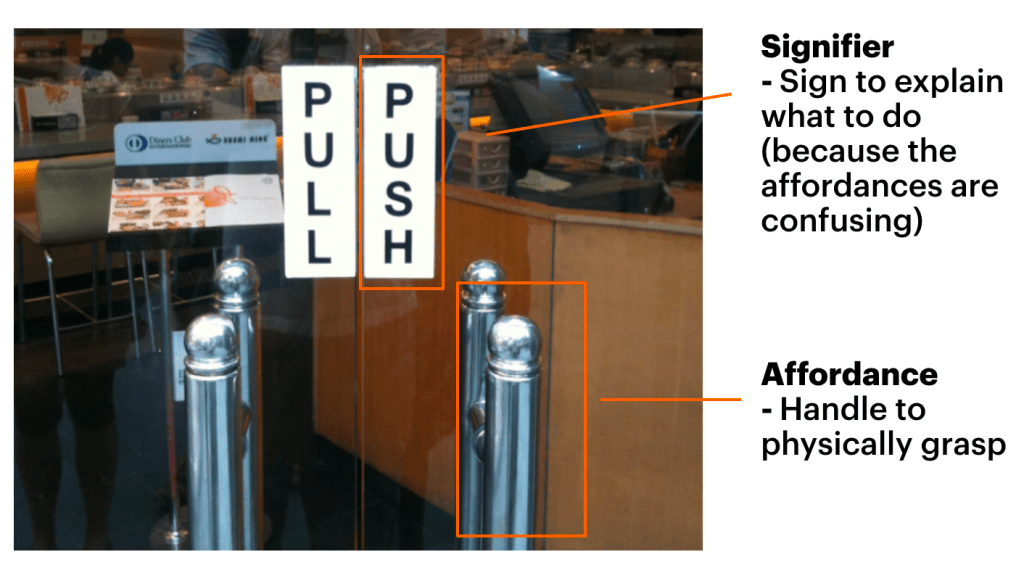
\includegraphics[width=0.5\textwidth]{affordance-vs-signifier.png}
    \caption{Affordance en signifier}
\end{figure}

\url{https://uxdesign.cc/what-is-an-affordance-6b60f2de79f2}


Vormen: 

\begin{itemize}
    \item Explicit affordance
    \item Pattern affordance
    \begin{itemize}
        \item Pattern metaphore
    \end{itemize}
    \item Hidden affordance
    \item False affordance
    \item Negative affordance
\end{itemize}


\subsection{Explicit affordance}
\begin{itemize}
    \item Een duidelijke affordance
    \item Door taal, bv: \underline{klik hier} om \dots $\Rightarrow$ signifiers
    \item Door hoe het er fysiek uitziet
    \item Makkelijk discoverable
\end{itemize}

\subsubsection{Voorbeelden}

\begin{itemize}
    \item `Click to play the video'
    \item Een grote knop met felle achtergrondkleur en subtiele 3d-vorm
\end{itemize}

\subsection{Pattern affordance}
\begin{itemize}
    \item Impliciet 
    \item Meest voorkomende type
    \item Maakt het mogelijk om in een complexe interface snel de interactieve onderdelen aan de gebruiker duidelijk te maken
    \item bv:
    \begin{itemize}
        \item Navigation bar
        \item Links
        \item Logo
        \item Link in bovenaan rechts
        \item Toggle switch
    \end{itemize}
\end{itemize}

\subsubsection{Pattern metaphors}

\begin{itemize}
    \item Metaforische affordance
    \item Real-world object als metafoor
    \item Icons
    \item Pattern metaforen
    \item Oppassen met heel herkenbare metaforen anders te designen.
\end{itemize}

\subsection{Hidden affordance}

\begin{itemize}
    \item Verborgen acties  
    \item Standaard wordt de affordance van een element pas onthuld als de gebruiker actie heeft ondernomen
    \item Om al complexe interfaces minder te clutteren
    \item Om minder belangrijke acties minder aandacht te geven
    \item bv:
    \begin{itemize}
        \item Reveal on hover
        \item Swipen van homescreen
    \end{itemize}
\end{itemize}

\subsection{False affordance}
\begin{itemize}
    \item Een woord dat onderlijnd is maar geen link is
    \item Een groene button die iets verwijderd
    \item Dark patterns?
    \item Een grijs woord waar op het eerste zicht geen actie achter zit maar toch een link of button is
    \item Om minder belangrijke acties minder aandacht te geven
\end{itemize}

\subsection{Negative affordance}

\begin{itemize}
    \item Soms is het nodig om aan te geven dat een UI-element op dit moment geen mogelijkheden biedt
    \item Grijze elementen
    \item Buttons die disabled zijn
\end{itemize}

\begin{figure}[H]
    \centering
    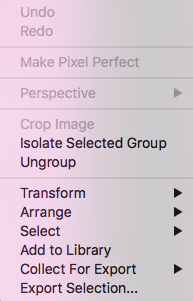
\includegraphics[width=0.5\textwidth]{negative-affordance.png}
    \caption{De grijze elementen zijn duidelijk niet klikbaar}
\end{figure}


\subsection{Overzicht}

\begin{figure}[H]
    \centering
    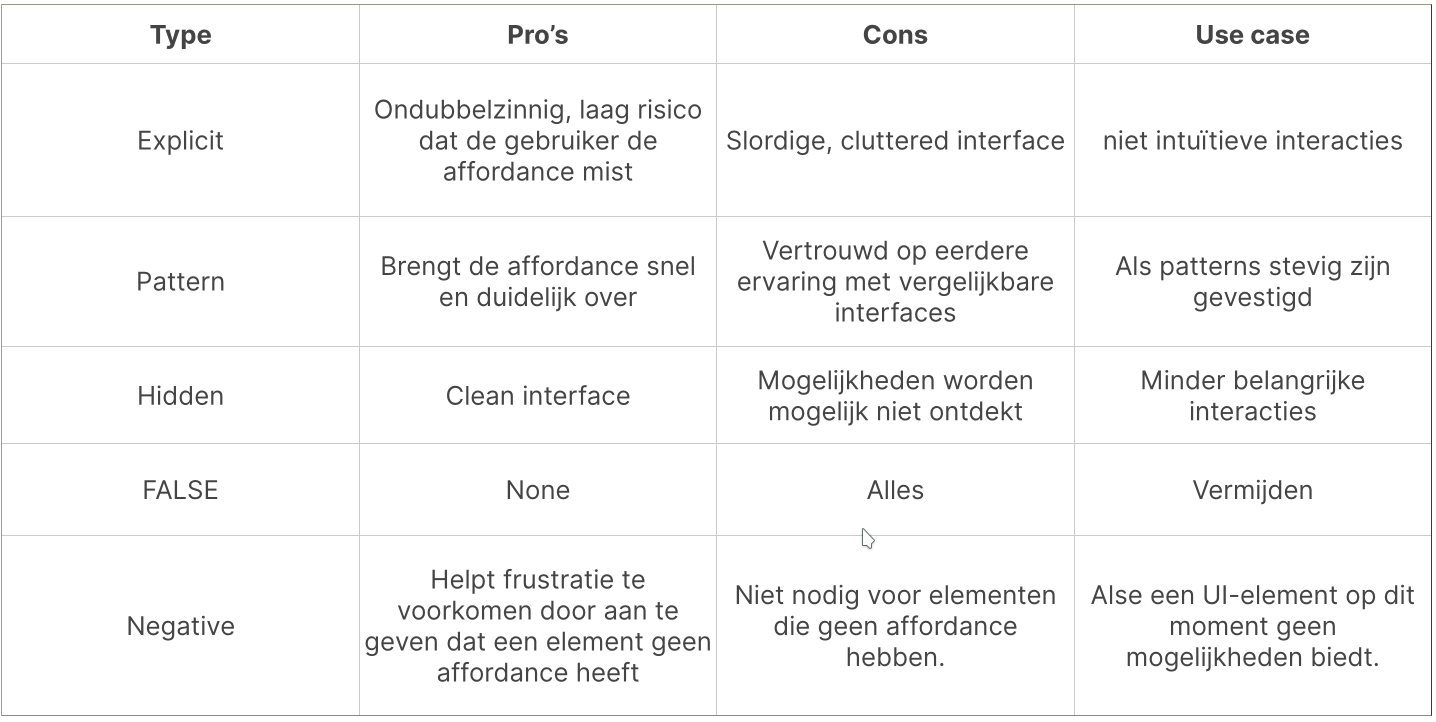
\includegraphics[width=0.9\textwidth]{affordance.png}
    \caption{Overzicht affordance}
\end{figure}



\section{Micro Interactions}

\subsection{Wat?}

\begin{itemize}
    \item Micro-interactions geven gebruikers onmiddellijke visuele feedback na het uitvoeren van een actie
    \item Ze wekken het vertrouwen op dat een uitgevoerde actie heeft plaatsgevonden en dat er als gevolg daarvan iets is gebeurd.
    \item Voegen een klein beetje `plezier' toe aan de UI
    \item Een klein interactief onderdeel van functionaliteit dat precies 1 iets doet
    \item \bold{Een hover effect is geen micro-interaction!}
\end{itemize}

\subsection{Actie - reactie - feedback}

Altijd 3 stappen: actie, reactie en feedback

\subsubsection{Voorbeeld: Toggle switch}

\begin{itemize}
    \item Actie: gebruiker duwt op de toggle switch om een setting af te zetten
    \item Reactie: setting wordt afgezet   
    \item Feedback: de toggle switch beweegt naar de andere kant, de achtergrondkleur verandert
\end{itemize}


\subsection{Versterkt door animatie}

\begin{itemize}
    \item Reactie en feedback is duidelijker
    \item Transition van de ene state naar de andere
    \item Maakt het verschil
\end{itemize}

\subsection{Waar gebruiken?}

\begin{itemize}
    \item Show system status
    \item Highlight changes
    \item Context behouden
    \item Calls to action
    \item Visualiseren van input
    \item Make tutorials come alive
    \item Foutmeldingen
    \item Succesmelding, voltooide acties
    \item Het tonen van veranderingen
\end{itemize}


\subsection{Voorbeelden}

\subsubsection{Iphone Mute}

\begin{itemize}
    \item Actie: user wil geluid op mute zetten op telefoon
    \item Reactie: geluid staat op stil, meldingen, bellen, etc
    \item Feedback: toestel vibreert
\end{itemize}

\subsubsection{Pull to refresh}

\begin{itemize}
    \item Actie: gebruiker trekt de pagina naar beneden
    \item Reactie: de pagina refresht
    \item Feedback: een refresh-icoontje verschijnt bovenaan de pagina
\end{itemize}

\subsubsection{Nightmode}

\begin{itemize}
    \item Actie: het wordt donker
    \item Reactie: Modus wordt aangepast
    \item Feedback: kleuren veranderen, helderheid wordt aangepast
\end{itemize}

\subsubsection{Facebook like}

\begin{itemize}
    \item Onderverdeling feedback
    \begin{itemize}
        \item Uitgebreid: comment
        \item Beknopt: Like
    \end{itemize}
    \item Microinteraction die legendarisch is geworden
\end{itemize}

\subsection{Combinaties van micro-interacties}

\begin{itemize}
    \item Meerdere micro-interactions maken een geheel en tonen wat er volgt op elkaar, en wat de actie ten gevolg heeft.
\end{itemize}

\subsection{Verandering aanduiden}

Duidelijke feedback bij:

\begin{itemize}
    \item Voltooiing van todo
    \item Verbergen van todo
\end{itemize}

\subsection{Don't}

\begin{itemize}
    \item Niet overdrijven
    \item Draagt de interactie bij aan het geheel
    \item Is de animatie niet storend
    \item Geen micro-interaction maken als er geen/weinig interactie is van de gebruiker
\end{itemize}

\subsection{Meer dan visuele feedback}

\begin{itemize}
    \item Geluid is een belangrijk deel van interactie
    \item Rekening houden met mute-state
    \item Met mate \& subtiel
\end{itemize}

\subsection{Resources}

\begin{itemize}
    \item \url{http://microinteractions.com/downloads/Microinteractions_Full_Color_Edition_excerpt.pdf}
    \item \url{https://vimeo.com/91559869}
    \item \url{http://microinteractions.com/what-is-a-microinteraction/}
    \item \url{https://dribbble.com/shots/2306244-Hoverboard-shop}
    \item \url{https://dribbble.com/shots/3167358-Microinteractions-for-to-do-list-app}
    \item \url{http://www.uiparade.com/portfolio/simple-toggle/}
    \item \url{https://uxplanet.org/best-practices-for-microinteractions-9456211aeed0}
    \item \url{https://techcrunch.com/2015/08/07/google-maps-new-night-mode-feature-makes-it-easier-to-navigate-in-the-dark/}
    \item \url{https://www.webdesignerdepot.com/2015/07/7-secrets-for-enhancing-ux-with-micro-interactions/}
    \item \url{http://zurb.com/blog/you-re-thinking-too-big-create-impact-wit}
    \item \url{https://dribbble.com/shots/2764222-Event-App-Concept}
    \item \url{https://dribbble.com/shots/1797373-Pull-Down-To-Refresh}
    \item \url{https://material.io/guidelines/motion/material-motion.html}
    \item \url{https://uxplanet.org/best-practices-for-microinteractions-9456211aeed0}
    \item \url{https://www.facebook.com/360Connext/photos/a.514490188584653.119917.217283351638673/649673881732949/?type=3&theater}
    \item \url{https://dribbble.com/shots/2174325-Alcatel-Watch-IA-Diagram/attachments/400188}
\end{itemize}


\section{API-calls, JavaScript basics \& debugging}

\subsection{JavaScript}

\begin{itemize}
    \item Enige client side manier om op het web te werken
    \item Is ge"evolueerd tot mogelijke full-stack oplossing
    \item Single thread, never blocking $\Rightarrow$ \underline{asynchrone} manier van werken
\end{itemize}

\subsubsection{Manier van werken}

\begin{enumerate}
    \item DOM element in een variabele stoppen
    \item Eventlistener (interactie), trigger
    \item In de eventlistener functie: inhoud schrijven, actie ondernemen
\end{enumerate}

\begin{figure}[H]
    \centering
    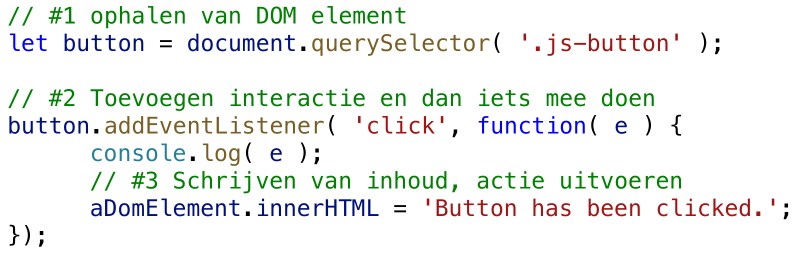
\includegraphics[width=0.5\textwidth]{js-manier-van-werken.png}
    \caption{Manier van werken}
\end{figure}

\subsubsection{Beschikbare structuren}

\begin{itemize}
    \item Objecten (data gestructureerd met naam bijhouden)
    \item Arrays (behouden een element met een bepaalde positie/nummer)
\end{itemize}

\begin{lstlisting}
let anObject = {
    fork: 'Fork'
}

let anArray = ['Fork', 'Spoon'];
\end{lstlisting}


\subsection{API calls in JS}

\subsubsection{Data ophalen in JS}
\begin{itemize}
    \item Via de fetch API
    \item Fetch API returns een promise (belofte)
\end{itemize}

\begin{lstlisting}
const serverendpoint = "https://api.example.com/v1/endpoint"

// GET
fetch(serverEndPoint)
    .then(function (response) {
        console.log(response);
        return response.json();
    })
    .then(function (json) {
        // Callback
        console.log(JSON.stringify(json));
    });
\end{lstlisting}

\subsubsection{Async/await functie}

\begin{itemize}
    \item In een async functie kunnen we een promise afwachten
    \item Vanaf dat moment kan je weer met een callback werken indien gewenst
    \item In plaats van `.then' gebruik je `await', met `async' in de functiedeclaration
\end{itemize}

\begin{lstlisting}
const getAPINewWay = async function() {
    const get = await fetch(serverEndPoint, { headers: headers });
    const joke = await get.json();
    console.log({ joke });
};
\end{lstlisting}

Kan nog beter: we kunnen de promise pas afwachten als de tweede \bold{`then'} voltooid is

\begin{lstlisting}
const data = await fetchData(serverEndPoint);
\end{lstlisting}

\subsubsection{Error handling}

Op deze laatste manier van schrijven is de .catch niet beschikbaar om te gebruiken.
Meest eenvoudige manier om op te lossen: alles in een try-catch block zetten.
Later maken we sowieso een class voor data-access, authentication, etc\dots


\subsection{Debugging}

\subsubsection{Logging}
\begin{lstlisting}
console.log({myVariable, anotherOne});
console.table([arrItems]); // voor arrays kan je console.table() gebruiken
\end{lstlisting}

\subsubsection{Browser breakpoints}

In de browser kan je breakpoints zetten om de code op een bepaalde lijn te stoppen, en lijn per lijn te overlopen.
Het is ook mogelijk om in de browser (snel) elementen op te vragen en te wijzigen.


\section{Animation}

\subsection{Transitions}

\begin{itemize}
    \item Geanimeerde verandering tussen 2 states
    \item User interaction
    \item Belangrijk onderdeel van User Interface design
    \item Micro interactions: hover, clicks, taps, gestures, \dots
    \item \url{https://codepen.io/rachelcope/pen/raGwPq}
    \item \url{https://tympanus.net/Development/Animocons/}
\end{itemize}

\subsection{Animations}

\begin{itemize}
    \item Een getimede animatie, heeft een start en een einde
    \item Start zonder dat de user iets doet
    \item De user kan er ook niets aan doen
    \item Eventueel pauzeren of stoppen
    \item \url{https://codepen.io/chrisgannon/pen/EjVyXN}
    \item \url{https://codepen.io/sol0mka/pen/ogOYJj}
\end{itemize}



\subsection{Speed}

Wordt bepaald door: 

\begin{itemize}
    \item Duration
    \item Easing
\end{itemize}

\subsection{Duration}

\begin{itemize}
    \item Hoe lang duurt de perfecte transition?
    \item Niet te lang en niet te kort
    \item Tussen 200ms en 500ms voor interface elementen
    \item Onder de 100ms zie je nauwelijks
    \item Boven de 1s is te traag en hinderlijk
    \item Afhankelijk van:
    \begin{itemize}
        \item Grootte object
        \item Afstand die ze afleggen
        \item Complexiteit
        \item Schermgrootte
    \end{itemize}
\end{itemize}

\bold{Tips}

\begin{itemize}
    \item Selection controls have a duration of 100ms:
    \item \url{https://material.io/design/motion/speed.html#duration}
    \item Animated elements that traverse a large portion of the screen have the longest durations
    \item \url{https://uxdesign.cc/the-ultimate-guide-to-proper-use-of-animation-in-ux-10bd98614fa9}
\end{itemize}

\begin{figure}[H]
    \centering
    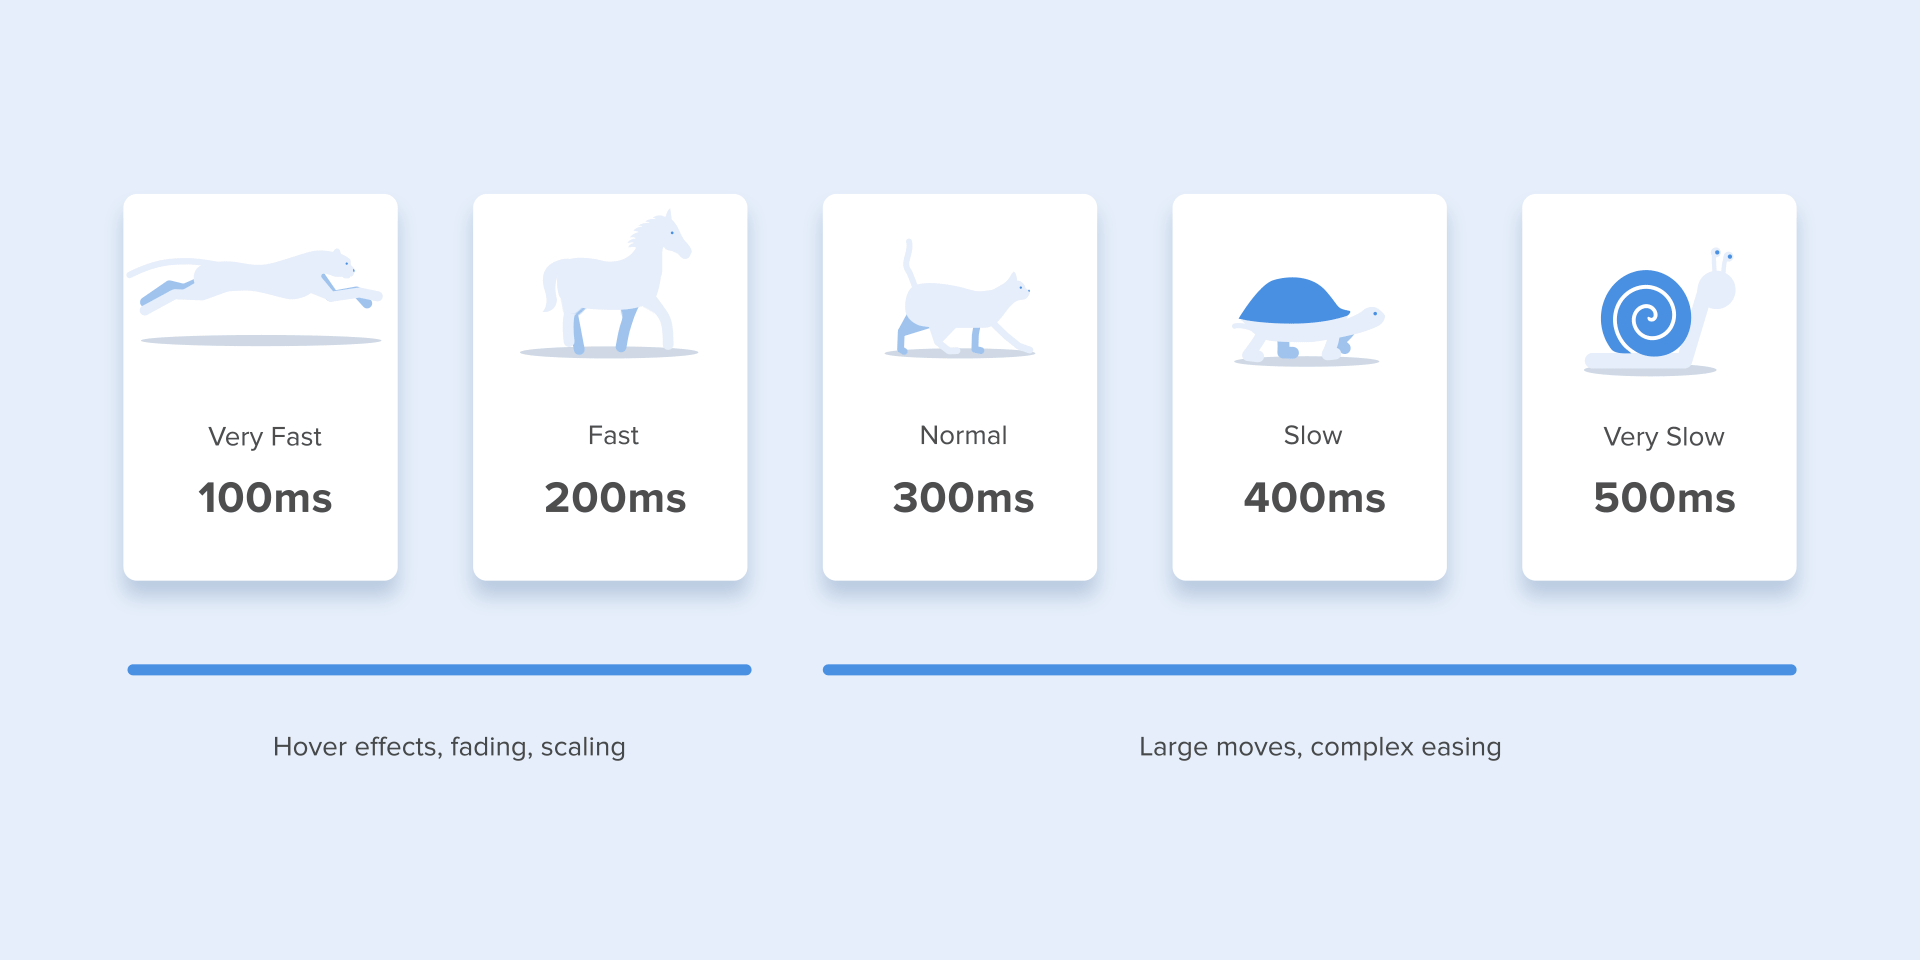
\includegraphics[width=0.7\textwidth]{animation-duration.png}
    \caption{}
\end{figure}

\subsection{Easing}

\begin{itemize}
    \item Progressie van de beweging over tijd (duration).
    \item Specificeert de versnelling of vertraging.
    \item Duration blijft hetzelfde.
    \item In plaats van een constant tempo (linear).
    \item Maakt de animatie natuurlijker.
    \item Geeft de animatie karakter.
    \item Alsof elementen beïnvloed worden door natuurlijke krachten zoals wrijving en zwaartekracht.
    \item 1 van de essentiële principes van animatie:
    \item \url{https://vimeo.com/93206523}
\end{itemize}

\bold{Tips}

\begin{itemize}
    \item Transitions without easing look stiff and mechanical
    \item \url{https://material.io/design/motion/speed.html\#easing}
    \item \url{https://uxdesign.cc/the-ultimate-guide-to-proper-use-of-animation-in-ux-10bd98614fa9}
\end{itemize}


\subsubsection{Cubic-bezier curves}

\begin{itemize}
    \item Visualiseren de progressie van de beweging over tijd (duration).
    \item Timing functions
    \item 4 punten:
    \begin{itemize}
        \item p0 en p3 = begin en einde
        \item p1 en p2 = control points
    \end{itemize}
    \item cubic-bezier(x-p1, y-p1, x-p2, y-p2)
\end{itemize}

\bold{Voorbeelden}

\url{https://callmenick.com/dev/level-up-animations-cubic-bezier/}

\begin{figure}[H]
    \centering
    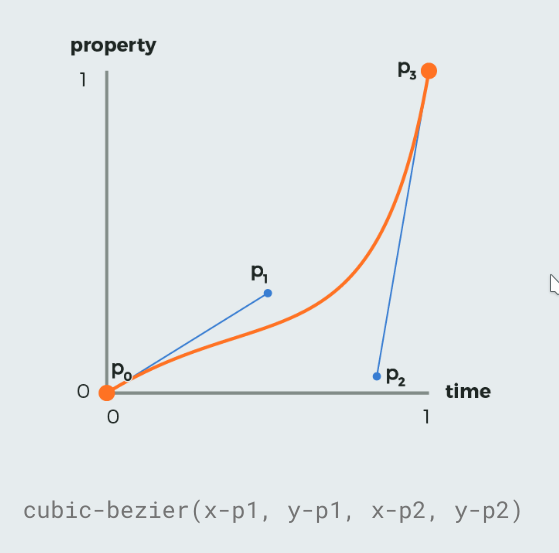
\includegraphics[width=0.4\textwidth]{animation-cubic-bezier.png}
    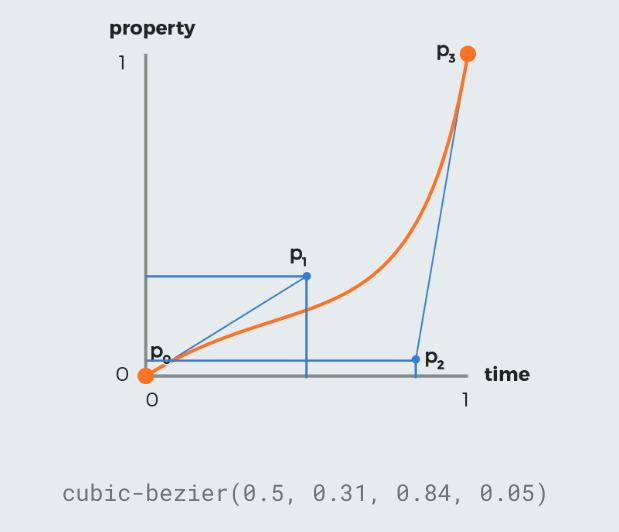
\includegraphics[width=0.47\textwidth]{animation-cubic-bezier2.png}
    \caption{Cubic-bezier function}
\end{figure}


\subsubsection{Ease-out}

\begin{itemize}
    \item Decelerate easing
    \item Begint snel, vertraagt naar het einde
    \item Ideaal voor inkomende elementen
\end{itemize}

\begin{figure}[H]
    \centering
    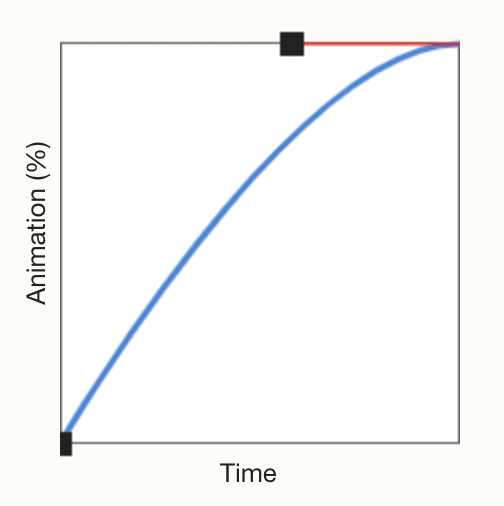
\includegraphics[width=0.2\textwidth]{animation-ease-out.png}
    \caption{Ease-out}
\end{figure}

\begin{figure}[H]
    \centering
    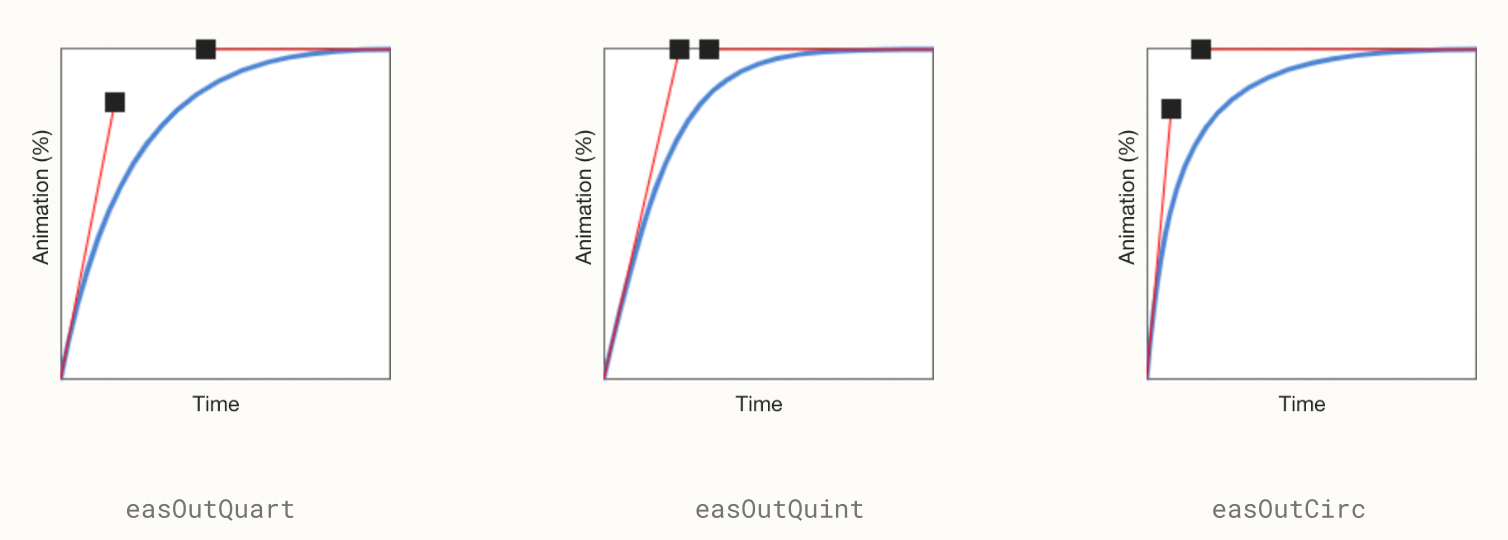
\includegraphics[width=0.6\textwidth]{animation-ease-out-extra.png}
    \caption{Ease-out extra functions}
\end{figure}

\begin{itemize}
    \item Accelerate easing
    \item Begint traag
    \item Versnelt naar het einde
    \item Ideaal voor uitgaande elementen
\end{itemize}

\begin{figure}[H]
    \centering
    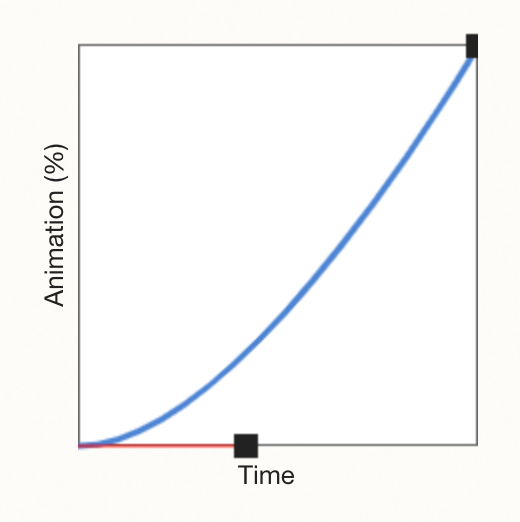
\includegraphics[width=0.2\textwidth]{animation-ease-in.png}
    \caption{Ease-in}
\end{figure}


\begin{figure}[H]
    \centering
    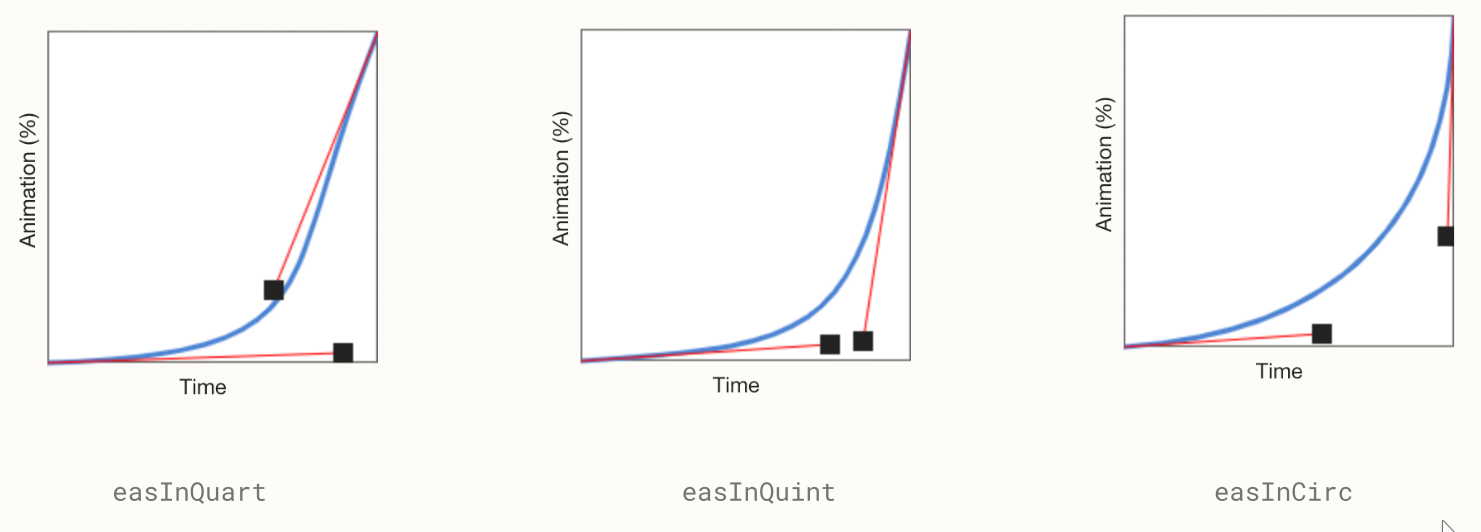
\includegraphics[width=0.6\textwidth]{animation-ease-in-extra.png}
    \caption{Ease-in extra functions}
\end{figure}

\subsubsection{Ease}

\begin{itemize}
    \item Meestvoorkomende soort easing
    \item Easing zowel op begin als einde
    \item Legt de nadruk op het einde van de animatie
    \item Geeft meer tijd aan de vertraging dan aan de versnelling.
\end{itemize}

\begin{figure}[H]
    \centering
    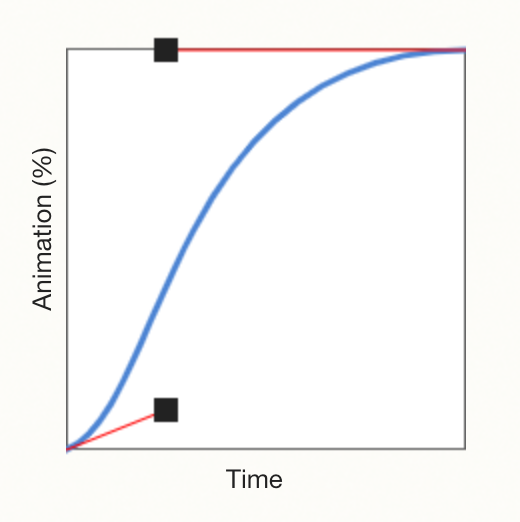
\includegraphics[width=0.4\textwidth]{animation-ease.png}
    \caption{}
\end{figure}


\subsubsection{Ease-in-out}

\begin{itemize}
    \item Begin en einde versnellen en vertragen even snel
    \item Tennis effect
    \item Heeft een specifiek karakter
    \item Ook niet voor elke situatie
\end{itemize}

\begin{figure}[H]
    \centering
    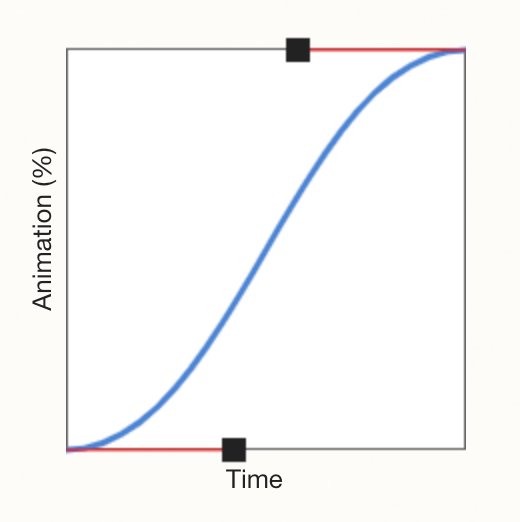
\includegraphics[width=0.4\textwidth]{animation-ease-in-out.png}
    \caption{Ease-in-out}
\end{figure}


\subsubsection{Ease-in-back en Ease-out-back}

\begin{itemize}
    \item \bold{Bounce effect}
    \item Maakt het nog levendiger (anticipation)
    \item Niet voor elke situatie
    \item Enkel voor beweging (niet voor color changes)
    \item Negatieve y-waarde
\end{itemize}

\begin{figure}[H]
    \centering
    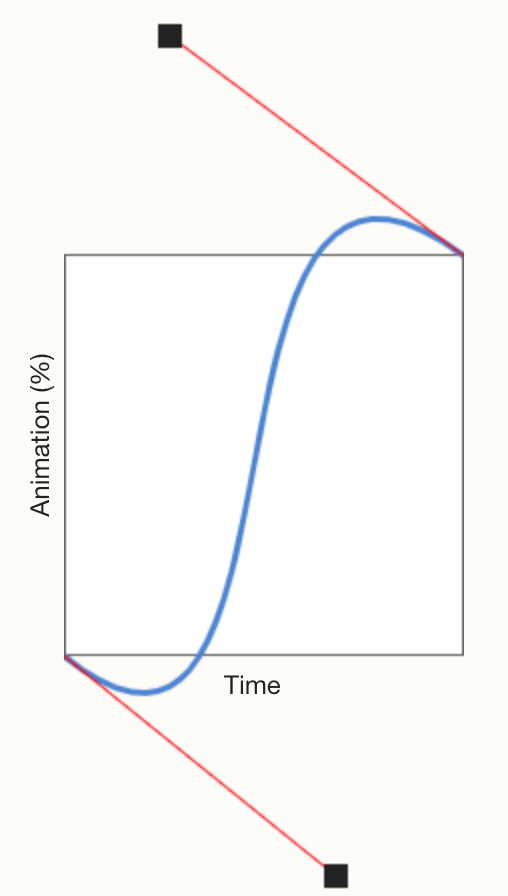
\includegraphics[width=0.35\textwidth]{ease-in-out-back.png}
    \caption{Ease-in/out-back}
\end{figure}




\subsection{CSS transition}
\begin{itemize}
    \item Automatische animatie tussen 2 verschillende property values.
    \item Keert automatisch terug als de animatie nog niet helemaal gedaan is
    \item Altijd op de initiële state declareren.
    \item \url{https://codepen.io/simoncoudeville-nmct/pen/bQNMQK}
\end{itemize}

\bold{Voorbeelden}

\begin{lstlisting}[language=CSS]
// Welke property er moet geanimeerd worden (default: all, optioneel)
transition-property: scale;

// duur van de animatie, in miliseconden of seconden
transition-duration: 300ms;

// easing (optioneel)
transition-timing-function: ease-in;

// vertraging vooraleer de animatie start
transition-delay: 1s;

// transition property: shorthand voor:
transition: [transition-property] [transition-duration] [transition-timing-function] [transition-delay];
\end{lstlisting}

\bold{Basic voorbeeld:}

\url{https://www.w3schools.com/cssref/tryit.asp?filename=trycss3_transition-property}

\subsubsection{Transition-timing-function}

\begin{itemize}
    \item Easing
    \item Standard easing names: (zijn ook cubic-bezier functions)
    \begin{itemize}
        \item ease (default)
        \item linear
        \item ease-in
        \item ease-out
        \item ease-in-out
    \end{itemize}
    \item Custom cubic-bezier (x-p1, y-p1, x-p2, y-p2)
    \item \url{https://matthewlein.com/tools/ceaser}
\end{itemize}

\bold{Transition-timing-function step values}

\begin{itemize}
    \item \bold{step-start:} the transition jumps instantly to the final state
    \item \bold{step-end:} the transtion stays at the initial state until the end, when it instantly jumps to the final state
    \item \bold{step(4, end):} by using steps() with an integer, you can define a specific number of steps before reaching the end.
    The state of the element will not vary gradually, but rather \bold{jump} from state to state in seperate instants
    \item \url{https://cssreference.io/property/transition-timing-function/}
    \item Wordt niet vaak gebruikt
\end{itemize}

\subsubsection{Multiple transitions}
\begin{lstlisting}[language=CSS]
transition: width 1s ease-in, height 2s ease-out, background-color 3s ease-in-out, transform 4s linear;

// of:

transition-property: width, height, background-color, transform;
transition-duration: 1s, 2s, 3s, 4s;
transition-timing-function: ease-in, ease-out, ease-in-out, linear;
\end{lstlisting}

\url{https://codepen.io/simoncoudeville-nmct/pen/rQOmGB}

\subsection{CSS animation}
\begin{itemize}
    \item Syntax om een getimede animatie in CSS te schrijven.
    \item Niet gebruiken voor transitions:
    \begin{itemize}
        \item Animations keren niet vanzelf terug: \url{https://codepen.io/simoncoudeville-nmct/pen/YRyQeJ}
    \end{itemize}
\end{itemize}

\subsubsection{Gelijkaardige properties:}

\begin{itemize}
    \item animation-duration
    \item animation-timing-function: werkt met dezelfde names en cubic-beziers.
    \begin{itemize}
        \item gebeurt per keyframe!
    \end{itemize}
\end{itemize}

\url{https://jaketrent.com/post/css-animation-timing-function-per-keyframe-segment/}

\subsubsection{Hoe maak je een CSS animation?}

\begin{itemize}
    \item Geef de animatie een naam
    \item Definieer de animation in @keyframes
    \item Roep de animation-naam op in een element en bepaal hoe het wordt geanimeerd.
    \item Basic voorbeeld: \url{https://codepen.io/simoncoudeville-nmct/pen/Zmbqvd}
\end{itemize}

\subsubsection{Zelfstudie}

\begin{itemize}
    \item \url{https://robots.thoughtbot.com/css-animation-for-beginners}
    \item \url{https://cssreference.io/property/animation-delay/}
    \item \url{https://codepen.io/collection/nbEZgX/}
\end{itemize}

\subsection{High performance animations}

\begin{itemize}
    \item \url{https://developer.mozilla.org/en-US/docs/Web/CSS/CSS_animated_properties}
    \item Welke properties kan je best gebruiken om te animeren?
    \item \url{https://www.html5rocks.com/en/tutorials/speed/high-performance-animations/}
    \item Als het kan:
    \begin{itemize}
        \item opacity
        \item transform: translate
        \item transform: rotate
        \item transform: scale
    \end{itemize}
    \item Gebruik de will-change property om de browser te waarschuwen wat geanimeerd zal worden    
\end{itemize}

\url{https://developers.google.com/web/fundamentals/design-and-ux/animations/animations-and-performance}

\url{https://medium.com/outsystems-experts/how-to-achieve-60-fps-animations-with-css3-db7b98610108}

\subsection{JavaScript libraries}

\begin{itemize}
    \item Niet alles is mogelijk met CSS
    \item Complexe easing functions
    \item Timeline control
    \item Transform properties apart animeren
    \item Complex sequencing
    \item Performantie
    \item Browser compatibility
    \item \dots
\end{itemize}

\subsubsection{Gsap}

\begin{itemize}
    \item \url{https://greensock.com/gsap/}
    \item \url{https://greensock.com/showcase}
\end{itemize}

\subsubsection{Anime.js}

\begin{itemize}
    \item \url{https://animejs.com/}
\end{itemize}

\subsubsection{Mo.js}

\begin{itemize}
    \item \url{https://github.com/mojs/mojs}
    \item \url{https://tympanus.net/Development/Animocons/}
\end{itemize}

\subsubsection{Popmotion}

\begin{itemize}
    \item \url{https://popmotion.io/}
\end{itemize}

\url{https://www.npmtrends.com/animejs-vs-gsap-vs-mo-js-vs-popmotion}

\subsubsection{Lottie + bodymovin}

\begin{itemize}
    \item Render After Effects animations natively on Web, Android and iOS, and React Native
    \item \url{https://github.com/airbnb/lottie-web}
    \item \url{http://airbnb.io/lottie/#/}
    \item \url{https://codepen.io/airnan/}
    \item Volgend semester in Web/App
\end{itemize}

\subsection{Oefening}

\begin{itemize}
    \item \url{https://codepen.io/simoncoudeville-nmct/pen/RqwzLw}
    \item Probeer de ball te laten springen zoals in het voorbeeld.
    \item Met high performance animation properties en de will-change property
\end{itemize}

\section{Grid Layout}

\subsection{Basics}

\begin{itemize}
    \item Flexbox = simpele 1-dimensionale layouts
    \item CSS Grid = comlexe 2-dimensionale layouts
    \begin{itemize}
        \item Columns \& Rows
        \item Global layouts, dashboards, \dots
        \item Krachtig en uitgebreid
    \end{itemize}
    \item Browser support: sinds 2017
    \item CSS tricks: \url{https://css-tricks.com/snippets/css/complete-guide-grid/#prop-grid-auto-columns-rows}
    \item Playground: \url{https://codepen.io/simoncoudeville-nmct/pen/JeMPPZ}
\end{itemize}

\subsubsection{Grid container}

= parent

\begin{itemize}
    \item Bepaalt de layout
    \item \url{https://codepen.io/simoncoudeville-nmct/pen/WNNPqQg}
\end{itemize}

\subsubsection{Grid layout}

\begin{itemize}
    \item Volgen de layout
    \item Default source order van de children maar laat toe om de order zowel verticaal als horizontaal te veranderen.
\end{itemize}

\begin{lstlisting}[language=HTML]
<!-- Container is de grid container -->
<div class="container">
    <div class="item item-1"></div>
    <div class="item item-2"></div>
    <div class="item item-3"></div>
</div>

<!-- Item elementen zijn grid-items. Subitems niet -->
<div class="container">
    <div class="item"></div>
    <div class="item">
        <p class="sub-item"></p>
    </div>
    <div class="item"></div>
</div>
\end{lstlisting}

\subsection{Grid line}

\begin{itemize}
    \item De scheidingslijnen die de structuur van het grid bepalen
    \item Vertical: column grid line
    \item Horizontal: row grid line
\end{itemize}

\begin{figure}[H]
    \centering
    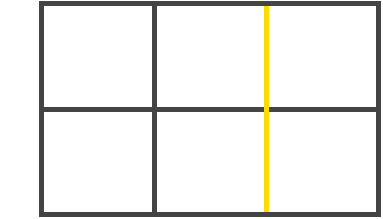
\includegraphics[width=0.3\textwidth]{grid-line-column.png}
    \caption{Column grid line}
\end{figure}

\subsection{Grid track}

\begin{itemize}
    \item De ruimte tussen 2 opeenvolgende grid lines
    \item Vertical: columns
    \item Horizontal: rows
\end{itemize}

\begin{figure}[H]
    \centering
    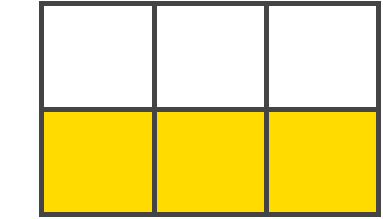
\includegraphics[width=0.3\textwidth]{grid-track.png}
    \caption{Grid track tussen de 2de en de 3de row grid lines}
\end{figure}

\subsection{Grid cell}

\begin{itemize}
    \item De ruimte tussen 2 opeenvolgende row \& column grid lines
\end{itemize}

\begin{figure}[H]
    \centering
    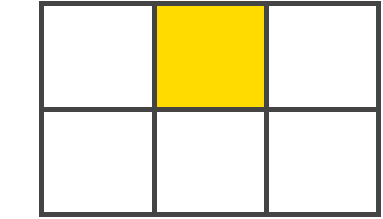
\includegraphics[width=0.3\textwidth]{grid-cell.png}
    \caption{Grid cell tussen row grid lines 1 \& 2, en column grid lines 2 \& 3.}
\end{figure}

\subsection{Grid area}

\begin{itemize}
    \item De ruimte tussen 2 row \& column grid lines
    \item Kan meerdere grid cells bevatten
\end{itemize}

\begin{figure}[H]
    \centering
    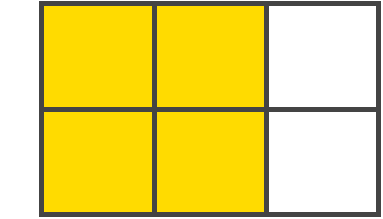
\includegraphics[width=0.3\textwidth]{grid-area.png}
    \caption{Grid area tussen row grid lines 1 \& 3, en column grid lines 1 \& 3.}
\end{figure}

\subsection{Properties}

\subsubsection{Properties voor de parent (grid container)}

\begin{itemize}
    \item display: grid | inline-grid
    \item \bold{Grid tracks, lines, en areas definieren: }
    \begin{itemize}
        \item grid-template-columns
        \item grid-template-rows
        \item grid-template-areas
        \item grid-template (shorthand)
    \end{itemize}
    \item \bold{Gap (gutter)}
    \begin{itemize}
        \item grid-column-gap
        \item grid-row-gap
        \item grid-gap (shorthand)
    \end{itemize}
    \item \bold{Alignment}
    \begin{itemize}
        \item justify-items
        \item align-items
        \item place-items
        \item justify-content
        \item align-content
        \item place-content
    \end{itemize}
    \item \bold{Auto-generated grid tracks}
    \begin{itemize}
        \item grid-auto-columns
        \item grid-auto-rows
        \item grid-auto-flow
    \end{itemize}
    \item grid: (shorthand)
\end{itemize}

\subsubsection{Properties voor de child (grid items)}

\begin{itemize}
    \item \bold{Locatie binnen de container}
    \begin{itemize}
        \item grid-column-start
        \item grid-column-end
        \item grid-row-start
        \item grid-row-end
        \item grid-column
        \item grid-row
        \item grid-area
    \end{itemize}
    \item \bold{Alignment:}
    \begin{itemize}
        \item justify-self
        \item align-self
        \item place-self
    \end{itemize}
\end{itemize}

\subsection{Grid-gap}
= De gutter tussen opeenvolgende items (niet links of rechts, boven of onder)

\begin{itemize}
    \item grid-column-gap: 4px;
    \item grid-row-gap: 8px; 
    \item grid-gap: <grid-row-gap> <grid-column-gap>
\end{itemize}

\subsection{Grid-template-columns en grid-template-rows}

\begin{itemize}
    \item Definieren de columns en rows
    \item Meerdere values gescheiden door spaties
    \item De values staan voor de track size
    \item De spaties staan voor de grid lines
\end{itemize}

\subsubsection{Syntax}

\begin{itemize}
    \item \bold{track-size:} auto, px, vh, vw, \% of een fraction van de overgebleven ruimte (\bold{fr})
    \item \bold{line-name:} automatische positieve en negatieve nummers. Maar je kan die zelf een naam geven om bij een item op te roepen
\end{itemize}

\subsubsection{Automatische line-names}

\begin{figure}[H]
    \centering
    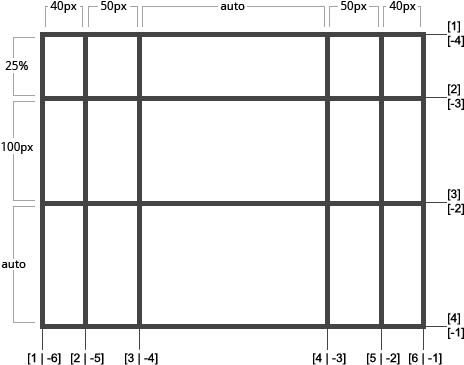
\includegraphics[width=0.4\textwidth]{grid-template.png}
    \caption{\bold{grid-template-columns}: 40px 50px auto 50px 40px; \\\bold{grid-template-rows}: 25\% 100px auto;}
\end{figure}

\begin{figure}[H]
    \centering
    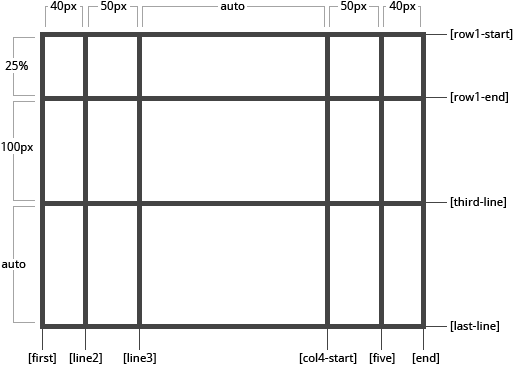
\includegraphics[width=0.4\textwidth]{grid-template-lines.png}
    \caption{\bold{grid-template-columns}: [first] 40px [line2] 50px [line3] auto [col4-start] 50px [five] 40px [end]; \\\bold{grid-template-rows}: [row1-start] 25\% [row1-end] 100px [third-line] auto [last-line];}
\end{figure}

\subsubsection{Track size special notations}

\begin{itemize}
    \item 1fr: fraction unit = 1 keer de overgebleven ruimte
    \item auto: neemt de breedste/hoogste content als basis voor de breedte/hoogte
    \item repeat(12, 1fr): maakt 12 kolommen aan van 1 fraction unit
    \item minmax(260px, 1fr): maakt 1 column of row aan van minimum 260px en maximum 1 fraction unit
    \item auto-fit en auto-fill keywords: responsive grid system zonder media queries!
    \item Combinaties: grid-template-columns: minmax(150px, 1fr) auto 1fr;
    \begin{itemize}
        \item Dit maakt 1 column aan van minimum 150px en maximum 1fr, 1 column die automatisch de breedte van de content krijgt en 1 column die altijd 1 fraction unit is.
    \end{itemize}
\end{itemize}

\subsubsection{grid-x-start, grid-x-end}
Waarbij x == column of row

\begin{itemize}
    \item Bepaalt de locatie van een grid items binnen het grid door te refereren naar grid lines
    \item Values:
    \begin{itemize}
        \item <line>: positief of negatief nummer of de zelfgekozen grid line name
        \item span <number> of <name>: hoeveel grid tracks moet het element innemen
    \end{itemize}
    \item Bijvoorbeeld: 
    \begin{itemize}
        \item grid-column-start: 2;
        \item grid-column-end: span 2;
        \item grid-column: 2 / span 2;
    \end{itemize}
\end{itemize}

\subsection{Grid-template-areas}

\begin{itemize}
    \item Laat toe om namen te geven aan grid areas
    \item Visuele representatie van je grid
    \item Values
    \begin{itemize}
        \item \bold{<grid-area-name>} =  een zelfgekozen naam
        \item \bold{.} = een lege grid cell
        \item \bold{none} = geen grid lines
    \end{itemize}
\end{itemize}

\subsubsection{Voorbeeld}

\begin{lstlisting}[language=CSS]
.container {
    grid-template-columns: 50px 50px 50px 50px;
    grid-template-rows: auto;
    grid-template-areas:
        "header header header header"
        "main main . sidebar"
        "footer footer footer footer";
}
\end{lstlisting}


\begin{figure}[H]
    \centering
    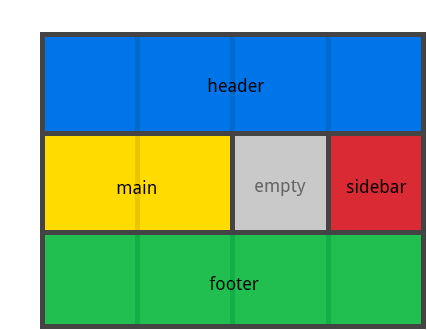
\includegraphics[width=0.5\textwidth]{grid-template-areas.png}
    \caption{Element met de .container class}
\end{figure}

\subsection{Grid-area}

\begin{itemize}
    \item Laat toe om een grid item op een \bold{voorgedefinieerde} grid area te plaatsen
    \item (Nog) een kortere manier dus om de volgorde te bepalen
\end{itemize}

\subsection{Voorbeelden}

\begin{itemize}
    \item CSS grid playground: \url{https://codepen.io/simoncoudeville-nmct/pen/JeMPPZ}
    \item Responsive dashboard grid: \url{https://codepen.io/simoncoudeville-nmct/pen/aQmENm}
\end{itemize}

\subsection{Zelfstudie}

\begin{itemize}
    \item \url{https://css-tricks.com/snippets/css/complete-guide-grid/}
    \item \url{https://dev.to/perborgen/want-to-learn-css-grid-here-s-my-free-full-length-course-31ln}
    \item \url{https://css-tricks.com/look-ma-no-media-queries-responsive-layouts-using-css-grid/}
    \item Auto-fill vs auto-fit: 
    \begin{itemize}
        \item \url{https://css-tricks.com/auto-sizing-columns-css-grid-auto-fill-vs-auto-fit/}
    \end{itemize}
    \item Minmax function:
    \begin{itemize}
        \item \url{https://bitsofco.de/how-the-minmax-function-works/}
    \end{itemize}
\end{itemize}

\subsection{Samenvatting: wat moet je weten?}

\begin{itemize}
    \item Waarom zou je CSS grid gebruiken ipv flexbox?
    \item Wat is een grid-area/-line/-cell?
    \item Met welke property bepaal je witruimte tussen 2 grid cells
    \item Waar staat fr voor? Wat is 1fr?
    \item Hoe maak je een grid met 12 kolommen die altijd even breed is?
    \item Auto-fill vs auto-fit?
\end{itemize}


\end{document}

